\باب{سوالات}

\حصہء{میکس ویل مساوات}
%====================
\ابتدا{سوال}
رداس \عددی{\rho=\SI{12}{\centi\meter}} کے گول دائرے میں وقت کے ساتھ تبدیل ہوتا، یکساں مقناطیسی میدان \عددی{B(t)=0.15\sin 1000 t \, \si{\weber}} ہے جو دائرے میں محرک برقی دباو \عددی{e(t)} پیدا کرتا ہے۔گول دائرے کی مزاحمت \عددی{\SI{55}{\ohm}} ہے۔محرک برقی دباو،  گول دائرے میں برقی رو \عددی{i(t)} پیدا کرتی ہے۔برقی رو \عددی{i(t)} سے پیدا مقناطیسی بہاو کو نظر انداز کرتے ہوئے \عددی{e(t)} اور \عددی{i(t)} حاصل کریں۔صورت حال شکل \حوالہ{شکل_سوال_میکس_ویل_دائرہ_محرک_دباو} میں دکھائی گئی ہے جہاں صفحہ سے اوپر کی جانب باہر نکلتی مقناطیسی میدان کو چھوٹے دائروں میں بند نقطوں سے ظاہر کیا گیا ہے۔
\begin{figure}
\centering
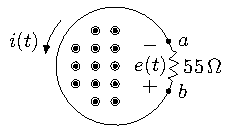
\includegraphics{figMaxwellRingEMF}
\caption{دائرے میں یکساں مقناطیسی بہاو، محرک برقی دباو پیدا کرتا ہے۔}
\label{شکل_سوال_میکس_ویل_دائرہ_محرک_دباو}
\end{figure}

جوابات:\عددی{-6.78 \cos 1000t \, \si{\volt}}، \عددی{-123\cos 1000t \, \si{\milli\ampere}}
\انتہا{سوال}
%======================
\ابتدا{سوال}
سطح \عددی{z=0} پر موصل تار کے مستطیل کے اطراف \عددی{x=\mp \SI{2}{\meter}}، \عددی{y=\mp\SI{1.5}{\meter}} پر ہیں۔وقت کے ساتھ تبدیل ہوتا مقناطیسی میدان \عددی{\kvec{B}=(0.25\ax-0.55\ay+0.1\az)\sin 1200 t \, \si{\tesla}} ہے۔مستطیل کی کل مزاحمت \عددی{R=\SI{4200}{\ohm}} ہے۔مثبت \عددی{z} محدد کی جانب سے دیکھتے ہوئے، گھڑی کی سمت میں برقی رو حاصل کریں۔برقی رو سے پیدا ثانوی مقناطیسی میدان کو نظر انداز کرتے ہوئے حل کریں۔

جواب:\عددی{343 \cos 1200 t \, \si{\milli\ampere}} 
\انتہا{سوال}
%=======================
\ابتدا{سوال}
مقناطیسی میدان \عددی{\kvec{B}=5\cos(1.2\times 10^{8} \pi t -\pi y)\az \, \si{\micro \tesla}} ہے۔مندرجہ ذیل فرضی یا غیر موصل دائروں پر \عددی{\aphi} سمت میں بڑھتا محرک برقی دباو حاصل کریں۔الف) \عددی{(0,0,0)} تا \عددی{(1,0,0)} تا \عددی{(1,1,0)} تا \عددی{(0,1,0)} تا \عددی{(0,0,0)}؛ ب) \عددی{(0,0,0)} تا \عددی{(2,0,0)} تا \عددی{(2,2,0)} تا \عددی{(0,2,0)} تا \عددی{(0,0,0)} 

جوابات:\عددی{600[\cos(1.2\times 10^{8} \pi t -\pi)-\cos (1.2 \times 10^{8} \pi t)] \, \si{\volt}}، \عددی{\SI{0}{\volt}}
\انتہا{سوال}
%=================
\ابتدا{سوال}
رداس \عددی{\rho=\SI{1}{\milli\meter}} اور \عددی{\rho=\SI{3}{\milli\meter}} کے ہم محوری تار
 میں \عددی{\kvec{H}=\tfrac{0.122}{\rho}\cos 5\times 10^{8} \pi t \cos 0.5 \pi z \aphi \, \si{\ampere\per\meter}} پایا جاتا ہے۔مستطیل \عددی{(0.001,0^{\circ},0)} تا \عددی{(0.003,0^{\circ},0)} تا \عددی{(0.003,0^{\circ},1.5)} تا \عددی{(0.001,0^{\circ},1.5)} تا \عددی{(0.001,0^{\circ},0)}   میں محرک برقی دباو حاصل کریں۔

جواب:\عددی{119\sin(5\times 10^{8}\pi t) \, \si{\volt}}
\انتہا{سوال}
%==================
\ابتدا{سوال}
لمحہ \عددی{t=0} پر موصل تار کے مستطیل کے اطراف \عددی{x=\SI{\mp 0.4}{\meter}} اور \عددی{y=\SI{\mp 0.6}{\meter}} پر ہیں۔یہ مستطیل \عددی{6 \ay \, \si{\meter\per\second}} کی سمتی رفتار سے حرکت کر رہی ہے۔غیر یکساں مقناطیسی میدان \عددی{\kvec{B}=3x^2y \az \, \si{\tesla}} ہے۔مستطیل کی مزاحمت \عددی{R=\SI{100}{\ohm}} ہے۔مستطیل میں طاقت کی اخراج حاصل کریں۔ساکن سلاخوں میں کتنی محرک برقی دباو پیدا ہوتی ہے۔  

جواب:\عددی{P=\SI{2.12}{\milli\watt}}، \عددی{\SI{0}{\volt}}
\انتہا{سوال}
%==================
\ابتدا{سوال}
شکل \حوالہ{شکل_میکس_ویل_سوال_محرک_سلاخ_ترچھی_ریل} میں دو ساکن موصل سلاخ \عددی{x} محدد کے ساتھ \عددی{\theta=\mp 10^{\circ}} کا زاویہ بناتے ہیں۔صفحہ کے بالائی سطح سے نکلتی مقناطیسی میدان \عددی{B=0.5\az \si{\tesla}} ہے۔ محرک سلاخ کی رفتار \عددی{v=8\ax \,\si{\meter\per\second}} ہے۔ ساکن سلاخوں کے بائیں سروں کے درمیان فاصلہ \عددی{\SI{2}{\centi\meter}} ہے۔ان کے مابین  آلہ پیما برقی دباو \عددی{v_{ab}} ناپتا ہے۔ الف) محرک سلاخ کے مقام کو \عددی{t=0} پر \عددی{x=0} لیتے ہوئے آلہ پیمائش پر حاصل برقی دباو کو مساوات \حوالہ{مساوات_میکس_ویل_فیراڈے_قانون} سے حاصل کریں۔ب)  اسی محرک دباو کو مساوات \حوالہ{مساوات_میکس_ویل_حرکت_سے_دباو} کے دائیں ہاتھ کی مدد سے حاصل کریں۔ پ) محرک سلاخ کا مقام \عددی{x=50t^2 \, \si{\meter\per\second}} ہونے کی صورت میں جواب حاصل کریں۔
\begin{figure}
\centering
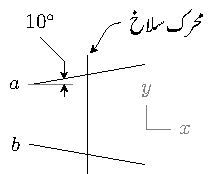
\includegraphics{figMaxwellSlidingConductorAngledRails}
\caption{محرک سلاخ پر مقناطیسی میدان محرک دباو پیدا کرتا ہے۔}
\label{شکل_میکس_ویل_سوال_محرک_سلاخ_ترچھی_ریل}
\end{figure}

جوابات:الف اور ب: \عددی{v_{ab}=-11.285t-0.08 \, \si{\volt}}، پ) \عددی{v_{ab}=-881.6t^3-t\, \si{\volt}} 
\انتہا{سوال}
%==================
\ابتدا{سوال}
رداس \عددی{\rho=\SI{0.5}{\centi\meter}} اور \عددی{\rho=\SI{4}{\centi\meter}} کی ہم محوری تار میں میدان \عددی{H_{\phi}=\tfrac{5}{\rho}\cos(2\pi\times 10^7 t - 5 z)} اور \عددی{E_{\rho}=\tfrac{8\pi^2}{\rho}\cos(2\pi \times 10^7 t -5z)} پائے جاتے ہیں۔ الف) مساوات \حوالہ{مساوات-میکس_ویل_تفرقی_الف} کے دونوں اطراف حل کرتے ہوئے ثابت کریں کہ ہم محوری تار میں موجود میدان اس پر پورا اترتے ہیں۔ ب) سمتی سطح \عددی{\phi=0}، \عددی{\SI{0.5}{\centi\meter} < \rho < \SI{4}{\centi\meter}}، \عددی{0<z<\SI{1}{\centi\meter}} اور اس کے محیط پر مساوات \حوالہ{مساوات_میکس_ویل_محرک_دباو_اور_گھٹاو_تعلق} کے دونوں اطراف حل کرتے ہوئے محرک برقی دباو حاصل کریں۔سمتی سطح کی سمت \عددی{\aphi} لیں۔یوں محیط پر چلتے ہوئے \عددی{z=\SI{1}{\centi\meter}} پر \عددی{\arho} سمت میں چلنا ہو گا۔    

جوابات:\عددی{\nabla  \times \kvec{E}=-\tfrac{\partial \kvec{B}}{\partial t}=\tfrac{40\pi^2}{\rho}\sin(2\pi \times 10^7 t - 5z)\aphi} ، \\ 
\عددی{\oint \kvec{E} \cdot \dif \kvec{L}=-\tfrac{\dif}{\dif t} \int \kvec{B} \cdot \dif \kvec{S}=52.26[\cos(2\pi \times 10^7 t -0.05)-\cos(2\pi \times 10^7 t)] \, \si{\volt}}
\انتہا{سوال}
%==================
\ابتدا{سوال}
شکل \حوالہ{شکل_میکس_ویل_سوال_کھلا_دور_بند_دور} میں \عددی{\kvec{B}=0.55\az \, \si{\tesla}} اور \عددی{\kvec{v}=6\ax\,\si{\meter\per\second}} ہیں۔محرک سلاخ میں انتہائی زیادہ مزاحمت رکھتا پیما برقی دباو \عددی{V} نسب ہے۔ الف) ساکن سلاخوں کے بائیں اور دائیں  سرے آزاد رکھتے ہوئے پیما پر کیا برقی دباو حاصل ہو گی۔ ب) ساکن سلاخوں کے بائیں سرے \عددی{a} اور \عددی{b} آپس میں موصل تار سے جوڑنے کے بعد پیما پر کیا حاصل ہو گا۔ پ) ساکن سلاخوں کے دائیں سرے آپس میں موصل تار سے جوڑنے کے بعد پیما پر کیا حاصل ہو گا۔ ت) ساکن سلاخ کے بائیں سرے آپس میں اور ان کے دائیں سرے آپس میں جوڑ کر پیما کیا پڑھے گا۔

\begin{figure}
\centering
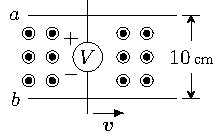
\includegraphics{figMaxwellSlidingConductorEndsOpen}
\caption{کھلے دور اور بند دور میں محرک برقی دباو۔}
\label{شکل_میکس_ویل_سوال_کھلا_دور_بند_دور}
\end{figure}

جوابات:\عددی{\SI{0}{\volt}}، \عددی{\SI{3.3}{\volt}}،  \عددی{\SI{3.3}{\volt}}، \عددی{\SI{3.3}{\volt}}
\انتہا{سوال}
%==================
\ابتدا{سوال}
برقی میدان \عددی{E=E_0 \cos 1500 t \, \si{\volt\per\meter}} کی صورت میں مندرجہ ذیل اشیاء میں ایصالی برقی رو اور انتقالی برقی رو کی شرح حاصل کریں۔ الف) تانبا جس کے مستقل \عددی{\epsilon_R=1} اور \عددی{\sigma=\SI{5.8e7}{\siemens\per\meter}} ہیں۔ ب) مقطر پانی جس کے مستقل \عددی{\epsilon_R=80} اور \عددی{\sigma=\SI{e-4}{\siemens\per\meter}} ہیں۔ پ) کوارٹس جس کے مستقل \عددی{\epsilon_R=3.8} اور \عددی{\sigma=\SI{e-17}{\siemens\per\meter}} ہیں۔

جوابات:\عددی{\tfrac{\sigma}{\omega \epsilon}}، \عددی{4.4\times 10^{15}}، \عددی{94}، \عددی{2\times 10^{-10}}
\انتہا{سوال}
%=================

\ابتدا{سوال}
برقی میدان \عددی{E=E_0 e^{\tfrac{t}{\tau}} \, \si{\volt\per\meter}} کی صورت میں مندرجہ ذیل اشیاء میں ایصالی برقی رو اور انتقالی برقی رو کی شرح حاصل کریں جہاں \عددی{\tau=10^{-7}} کے برابر ہے۔ الف) تانبا جس کے مستقل \عددی{\epsilon_R=1} اور \عددی{\sigma=\SI{5.8e7}{\siemens\per\meter}} ہیں۔ ب) مقطر پانی جس کے مستقل \عددی{\epsilon_R=80} اور \عددی{\sigma=\SI{e-4}{\siemens\per\meter}} ہیں۔ پ) کوارٹس جس کے مستقل \عددی{\epsilon_R=3.8} اور \عددی{\sigma=\SI{e-17}{\siemens\per\meter}} ہیں۔

جوابات:\عددی{\tfrac{\sigma \tau}{\epsilon}}، \عددی{\num{6.5e11}}، \عددی{\num{0.014}}، \عددی{\num{2.97e-11}}
\انتہا{سوال}
%=================
\ابتدا{سوال}
محدد \عددی{z} پر موجود ہم محوری تار کی لمبائی \عددی{\SI{12}{\centi\meter}} جبکہ اس کے رداس \عددی{\SI{2}{\milli\meter}} اور \عددی{\SI{6}{\milli\meter}} ہیں۔ دونوں تاروں کے درمیان مادے کے مستقل \عددی{\mu=\SI{5e-6}{\henry\per\meter}}، \عددی{\epsilon=\SI{2e-11}{\farad\per\meter}} اور \عددی{\sigma=\SI{4e-5}{\siemens\per\meter}} ہیں۔تار میں \عددی{\kvec{E}=\tfrac{10^4}{\rho}\cos (10^6t) \arho \, \si{\volt\per\meter}} کی صورت میں \عددی{\kvec{J}}، \عددی{I_c}، \عددی{\kvec{J}_d}، \عددی{I_d} اور \عددی{\tfrac{\abs{I_d}}{\abs{I_c}}} حاصل کریں۔

جوابات:\عددی{\tfrac{0.5}{\rho}\cos(10^6 t)\arho \, \si{\ampere\per\meter\squared}}، \عددی{0.12\pi\cos 10^6 t \, \si{\ampere}}، 
\عددی{-\tfrac{0.1}{\rho}\sin 10^6 t \, \si{\ampere\per\meter \squared}}، \عددی{-0.024\pi\sin 10^6 t \, \si{\ampere}}، \عددی{0.2}
\انتہا{سوال}
%==================
\ابتدا{سوال}
رداس \عددی{\rho_1} اور \عددی{\rho_2} کے ہم محوری تار کی لمبائی \عددی{l} ہے۔تار  کو بیرونی دور \عددی{V_0 \cos \omega t} برقی دباو فراہم کرتی ہے۔تار میں برقی میدان \عددی{\kvec{E}} کی مساوات لکھتے ہوئے \عددی{\kvec{J}_d} اور \عددی{I_d} حاصل کریں۔ثابت کریں کہ انتقالی برقی رو بیرونی دور میں پائی جانے والی ایصالی برقی رو کے برابر ہے۔

جوابات:\عددی{\kvec{E}=\tfrac{V_0\cos \omega t}{\rho \ln \tfrac{b}{a}}\arho \, \si{\volt\per\meter}}،
 \عددی{\kvec{J}_d=\tfrac{-\omega \epsilon V_0\sin \omega t}{\rho \ln \tfrac{b}{a}}\arho}،
  \عددی{I_d=-\tfrac{2\pi l \omega \epsilon V_0\sin \omega t}{\ln \tfrac{b}{a}}}،
 \عددی{I_c=C\tfrac{\dif V}{\dif t}=-\tfrac{2\pi l \omega \epsilon V_0\sin \omega t}{\ln \tfrac{b}{a}}}
\انتہا{سوال}
%=================
\ابتدا{سوال}
مساوات \حوالہ{مساوات-میکس_ویل_دوسری_مساوات_نقطہ_شکل_ب} کی پہلی مساوات کے دونوں اطراف پھیلاو کا عمل استعمال کرتے ہوئے  استمراری مساوات حاصل کریں۔

جواب:\عددی{\nabla \cdot \nabla \times \kvec{H}=0=\nabla \cdot \kvec{J}+\tfrac{\partial \rho_h }{\partial t}} 
\انتہا{سوال}
%====================
\ابتدا{سوال}
ایک خطہ جہاں \عددی{\kvec{E}=32\sin ax \cos 5y \cos (2\times 10^{10} t) \az} ہے کے مستقل \عددی{\mu_R=2.5}، \عددی{\epsilon_R=1.2} اور \عددی{\sigma=0} ہیں۔میکس ویل کے مساوات استعمال کرتے ہوئے \عددی{a} کی مثبت قیمت دریافت کریں۔تمام تکمل کے مستقل کو صفر لیں۔

جواب:\عددی{a=\SI{115.44}{\meter^{-1}}}
\انتہا{سوال}
%=====================
\ابتدا{سوال}
ایک ترسیلی تار میں مقناطیسی میدان \عددی{\kvec{H}=15\cos(4\times 10^9 t - \beta z) \ax \, \si{\ampere\per\meter}} پایا جاتا ہے۔ترسیلی تار کے درکار مستقل \عددی{\mu_R=1}، \عددی{\epsilon_R=5} اور \عددی{\sigma=0} ہیں۔میکس ویل کے مساوات استعمال کرتے ہوئے \عددی{\beta} کی مثبت قیمت دریافت کریں۔

جواب:\عددی{\beta=\SI{29.83}{\meter^{-1}}}
\انتہا{سوال}
%======================
\ابتدا{سوال}
موصل سطح محدد کے مرکز سے گزرتی ہے جہاں میدان \عددی{\kvec{E}=(33\ax+12\ay+25\az)\cos(10^7 t) \, \si{\volt\per\meter}} پایا جاتا ہے۔سطح کے قریب خطے کے مستقل \عددی{\sigma=0}، \عددی{\epsilon_R=12} اور \عددی{\mu_R=1.6} ہیں۔نقطہ \عددی{(0,0,0)} پر موصل سطح پہ کثافت چارج حاصل کریں۔اس نقطے پر سطح کے متوازی میدان حاصل کریں۔

جوابات:\عددی{4.58\cos(10^7 t) \, \si{\nano\coulomb\per\meter\squared}}، \عددی{0}
\انتہا{سوال}
%=====================
\ابتدا{سوال}
خطہ \عددی{z<0} میں \عددی{\epsilon_{R1}=1}، \عددی{\mu_{R1}=1} اور \عددی{\sigma_1=0} ہیں جبکہ خطہ \عددی{z>0} میں \عددی{\epsilon_{R2}=9}، \عددی{\mu_{R2}=4} اور \عددی{\sigma_2=0} ہیں۔پہلے خطے میں میدان \عددی{\kvec{E}_1=[10\cos(10^9t-3.336z)-2\cos(10^9t+3.336z)]\ay} اور دوسرے خطے میں \عددی{\kvec{E}_2=(A\cos(10^9t-20.014z))\ay} ہیں۔ الف) مستقل \عددی{A} کی قیمت دریافت کریں۔ ب) مقناطیسی میدان \عددی{\kvec{H}_1} اور \عددی{\kvec{H}_2} حاصل کریں۔ پ) ثابت کریں کہ مقناطیسی میدان سرحدی شرائط پر پورا اترتے ہیں۔

جوابات:\عددی{A=8}، \عددی{\kvec{H}_1=[-0.0265\cos(10^9t-3.336z)-0.0053\cos(10^9 t +3.336z)]\ax}،\\
 \عددی{\kvec{H}_2=-0.0318\cos(10^9 t -20.014z)\ax} ،\عددی{H_{m1}=H_{m2}}
\انتہا{سوال}
%=====================
\ابتدا{سوال}\شناخت{سوال_میکس_ویل_غیر_متوقع_میدان}
خالی خلاء میں مساوات \حوالہ{مساوات_میکس_ویل_غیر_حقیقی_میدان} نلکی محدد میں میدان دیتی ہے۔خالی خلاء میں \عددی{\kvec{J}=0} لیتے ہوئے میکس ویل کی مساوات \عددی{\nabla \times \kvec{H}=\kvec{J}+\tfrac{\partial \kvec{D}}{\partial t}} استعمال کرتے ہوئے \عددی{\kvec{E}} حاصل کریں۔حاصل \عددی{\kvec{E}} سے میکس ویل کی مساوات \عددی{\nabla \times \kvec{E}=-\tfrac{\partial \kvec{B}}{\partial t}} کی مدد سے  واپس \عددی{\kvec{B}} حاصل کریں۔یوں ثابت کریں کہ دی گئی میدان میکس ویل کی مساوات پر پورا نہیں اترتا۔ 

جواب:چونکہ ہمیں واپس ابتدائی میدان حاصل نہیں ہوتا لہٰذا یہ میدان میکس ویل کی مساوات پر پورا نہیں اترتا۔
\انتہا{سوال}
%====================
